\chapter{\ifproject%
\ifenglish Project Structure and Methodology\else โครงสร้างและขั้นตอนการทำงาน\fi
\else%
\ifenglish Project Structure\else โครงสร้างของโครงงาน\fi
\fi
}

ในบทนี้จะกล่าวถึงหลักการ และการออกแบบระบบ

\makeatletter

% \renewcommand\section{\@startsection {section}{1}{\z@}%
%                                    {13.5ex \@plus -1ex \@minus -.2ex}%
%                                    {2.3ex \@plus.2ex}%
%                                    {\normalfont\large\bfseries}}

\makeatother
%\vspace{2ex}
% \titleformat{\section}{\normalfont\bfseries}{\thesection}{1em}{}
% \titlespacing*{\section}{0pt}{10ex}{0pt}

\section{ขั้นตอนการดําเนินงาน}

\subsection{ขั้นตอนการเก็บ requirements}
\subsubsection{สำหรวจปัญหาจากการสอบถาม}
การสําหรวจจากการสอบถามของตัวแทนนักศึกษา 10 คน โดยมีวัตถุประสงค์เพื่อแก้ปัญหาต่างๆในการใช้
ชีวิตในมหาวิทยาลัย โดยเน้นไปที่การช่วยเหลือนักศึกษาใหม่ที่เป็นช่วงในการปรับตัวเข้ากับสังคมในมหาวิทยาลัย

\subsubsection{วิเคราะห์ปัญหา}
สามารถสรุปได้เป็นประเด็นดังนี้
\begin{enumerate}
  \item การที่เราอยากรู้ถึงวิธีการแก้ปัญหาที่เราเผชิญอยู่นั้นการค้นหาข้อมูลจากอินเทอร์เน็ต โดยส่วนมากการ
  ค้นหาข้อมูลที่มีลักษณะ เป็นประสบการณ์จากคนที่เคยแก้ปัญหาเรื่องนั้นมาก่อน บางครั้งการค้นหา
  ข้อมูลลักษณะนี้มักจะหาข้อมูลได้ยาก การใช้คําในการค้นหา ข้อมูลกระจายไปในที่ต่างๆหลากหลาย
  เวปไชต์ยิ่งต้องใช้เวลาในการเพิ่มไปอีก นอกจากนี้ยิ่งเป็นเรื่องราวเฉพาะพื้นที่ทําให้ข้อมูลยิ่งหายากมาก
  ขึ้น
  \item การขอคําปรึกษาจากผู้ที่เรารู้จักนั้น บางครั้งอาจจะได้คําตอบที่ไม่ตรงกับที่คาดหวังอาจเนื่องมาจากผู้
  ที่เราขอความช่วยเหลื่อไม่มีความรู้หรือประสบการในเรื่องนั้น
  
  \item การสอบคําถามนั้นบางครั้งผู้ถามอาจจะเกิดความเขินอายในการที่จะถามในเรื่องนั้นออกไป ทําให้ไม่
  ความความกล้าในการขอความช่วยเหลือ
  
  \item ในกรณีของนักศึกษาใหม่การหาหอพัก สวัสดิการช่วยเหลือของมหาลัยไม่ค่อยเป็นที่พูดถึงในโชเชียลมา
  กนัก บางครั้งอาจได้รับข้อมูลที่ผิดจากคนที่ไม่มีประสบการณ์และไม่รู้จริง
\end{enumerate}

\subsubsection{สรุปปัญหาหาแนวทางแก้ไขและออกแบบ}
\begin{enumerate}
  \item ออกแบบแอปพลิเคชันที่สามารถเป็นสื่อกลางในการรวบรวมประสบการณ์ต่างๆจากการรีวิว มีการแบ่ง
  เป็นหมวดหมู่สามารถเข้าถึงได้ง่าย ซึ่งตัวแอปพลิเคชันจะมีวัตถุประสงค์ในการช่วยเหลือนักศึกษามหาวิทยาลัยเชียงใหม่ทําให้มีลักษณะของการรวมคนเฉพาะพื้นที
  
  \item ในเรื่องของความน่าเชื่อถือของการีวิวสามารถดูได้จากคะแนนการรีวิวยิ่งคะแนนมาก ความน่าเชื่อถือ
  ยิ่งมาก
  \item สามารถถามคําถามเพื่อหาคนที่เราสามารถขอคําปรึกษาจากผู้ที่รู้และมีประสบการณ์ในเรื่องนั้นๆ
  \item สามารถปิดบังตัวตนเพื่อเพิ่มความกล้าในการขอความช่วยเหลือ
\end{enumerate}

\subsubsection{ขั้นตอนการออกแบบระบบ}
\begin{enumerate}
  \item ออกแบบ Use case diagram
  \item เลือกเทคโนโลยีและเครื่องมือที่จะใช้
  
  \item  ออกแบบ UI ใน Figma โดยมีพื้นฐานการออกแบบมาจากการใช้งานแอปพลิชันโซเชียลมีเดียทั่วไป
  
\end{enumerate}
\section{โครงสร้างของแอปพลิเคชัน}
\subsection{Use case diagram}
แสดงให้เห็นภาพรวมของการใช้งานระบบดังรูปที่ 3.1 จาก requirement เราสามารถระบุUser คือกลุ่ม
บุคคลที่ใช้แอปพลิเคชันทั่วไป เมื่อเข้าสู่ระบบมาแล้วสามารถเข้าถึง Use case ต่างๆได้ดังนี้
\begin{enumerate}
  \item การรีวิว สามารถสร้างการีวิวเรื่องต่างๆ สามารถเข้ามาอ่านการรีวิว สามารถคอมเม้นและให้คะแนน
  การรีวิว
  \item กระดานตั้งกระทู้ถาม-ตอบ สามารถเข้าอ่าน ช่วยตอบข้อสงสังต่างๆผ่านการดานถามตอบปัญหาหรือ
  สร้างกระทู้ถามคําถามเองก็ได้
  \item  ระบบสนทนา สามารถเเชทเพื่อปรึกษาหารือกันได้

\end{enumerate}
\begin{figure}[ht]
  \begin{center}
    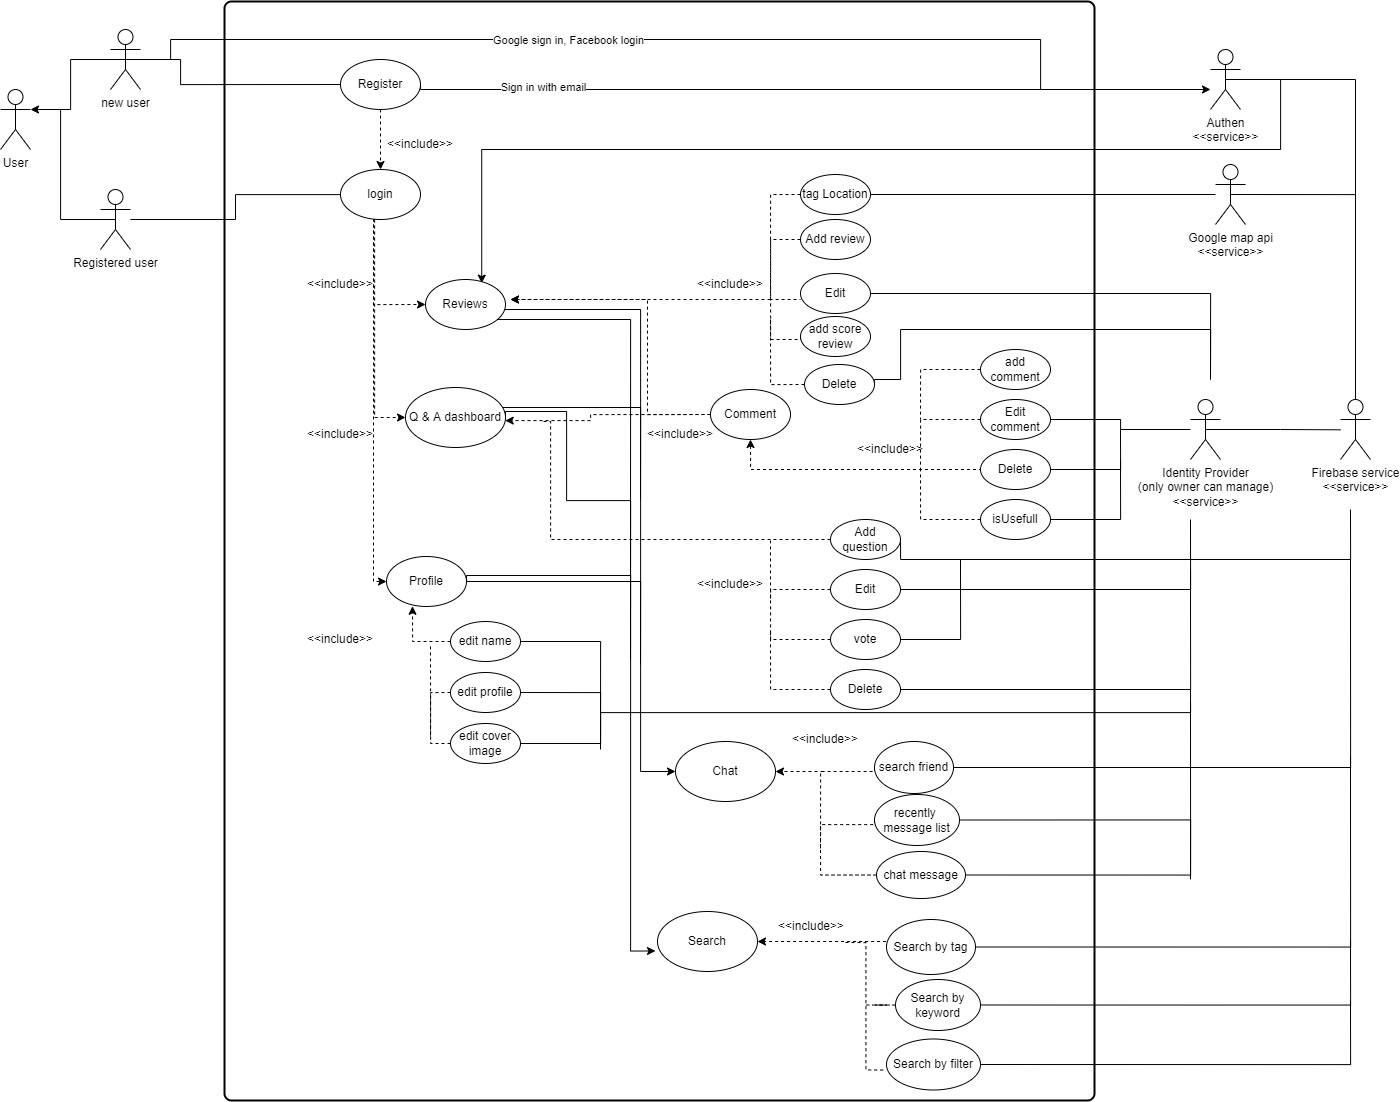
\includegraphics[width=1\textwidth]{./image/user-diagram.jpg}
  \end{center}
  \caption[Poem]{Use case diagram}
  \end{figure}

\subsection{System architecture}
สถาปัตยกรรมโครงสร้างของระบบในส่วนของการแสดงผลของ mobile application จะใช้java ในการเขียนแอพพลิเคชันและเชื่อมต่อ backend ด้วย firebase โดยบริการที่ใช้ของfirebaseได้แก่ Realtime Database
,Authentication และ Storage 

การลงชื่อเข้าใจสามารถลงชื่อผ่านแพลตฟอร์มอื่นได้ เช่น google(ผ่าน firebase Authentication) ,facebook(ผ่าน facebook api) ข้อมูลที่ใช้ในระบบจะถูกเก็บไว้ในฐานข้อมูล
บน firebase realtime ส่วนการเก็บข้อมูลของรูปภาพจะเก็บไว้ที่ firebase storage สามารถแท็ก location ที่อยู่บน google map  ดังรูปที่ 3.2  

\begin{figure}[ht]
  \begin{center}
    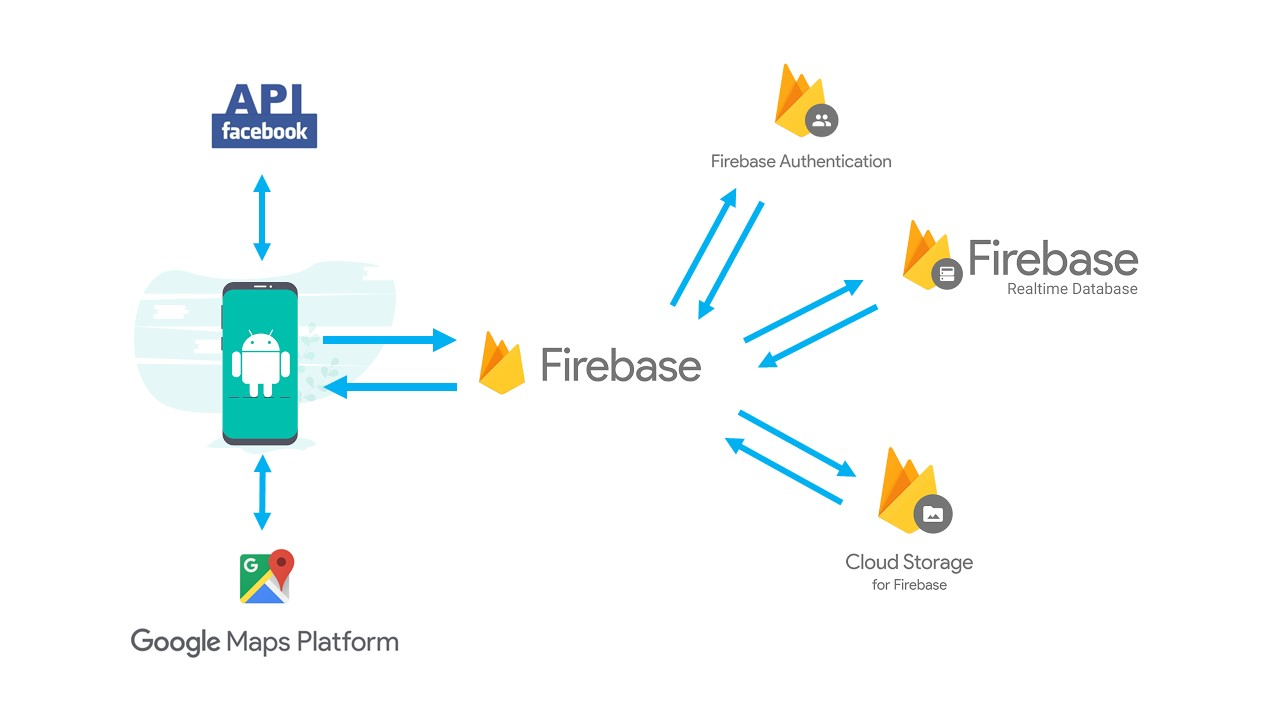
\includegraphics[width=0.9\textwidth]{./image/structure.jpg}
  \end{center}
  \caption[Poem]{System architecture}
  \end{figure}

\newpage
\subsection{Database schema}
 การเก็บข้อมูลในรูปแบบ NoSQL เก็บเป็น collections ต่างๆ ดังรูปที่ 3.3 
\begin{enumerate}
  \item Users จะเก็บข้อมูลของผู้ใช้
  \item Reviews จะเก็บข้อมูลของการรีวิว
  \item Rparticipation เก็บข้อมูลการมีส่วนร่วมกับ Reviews เช่น การให้คะแนนรีวิว
  \item QuestionAns จะเก็บข้อมูลของการกระดานถาม-ตอบ
  \item Qparticipation เก็บข้อมูลการมีส่วนร่วมกับ QuestionAns เช่น การกดถูกใจ
  \item MyLocation เก็บรายละเอียดของตำแหน่งที่ตั้ง
  \item Comments จะเก็บข้อมูลของคอมเมนต์
  \item MessageList จะเก็บข้อมูลของรายชื่อผู้รับ-ผู้ส่ง
  \item Chats จะเก็บข้อมูลรายละเอียดเนื้อหาการสนทนา
\end{enumerate}
\begin{figure}[ht]
  \begin{center}
    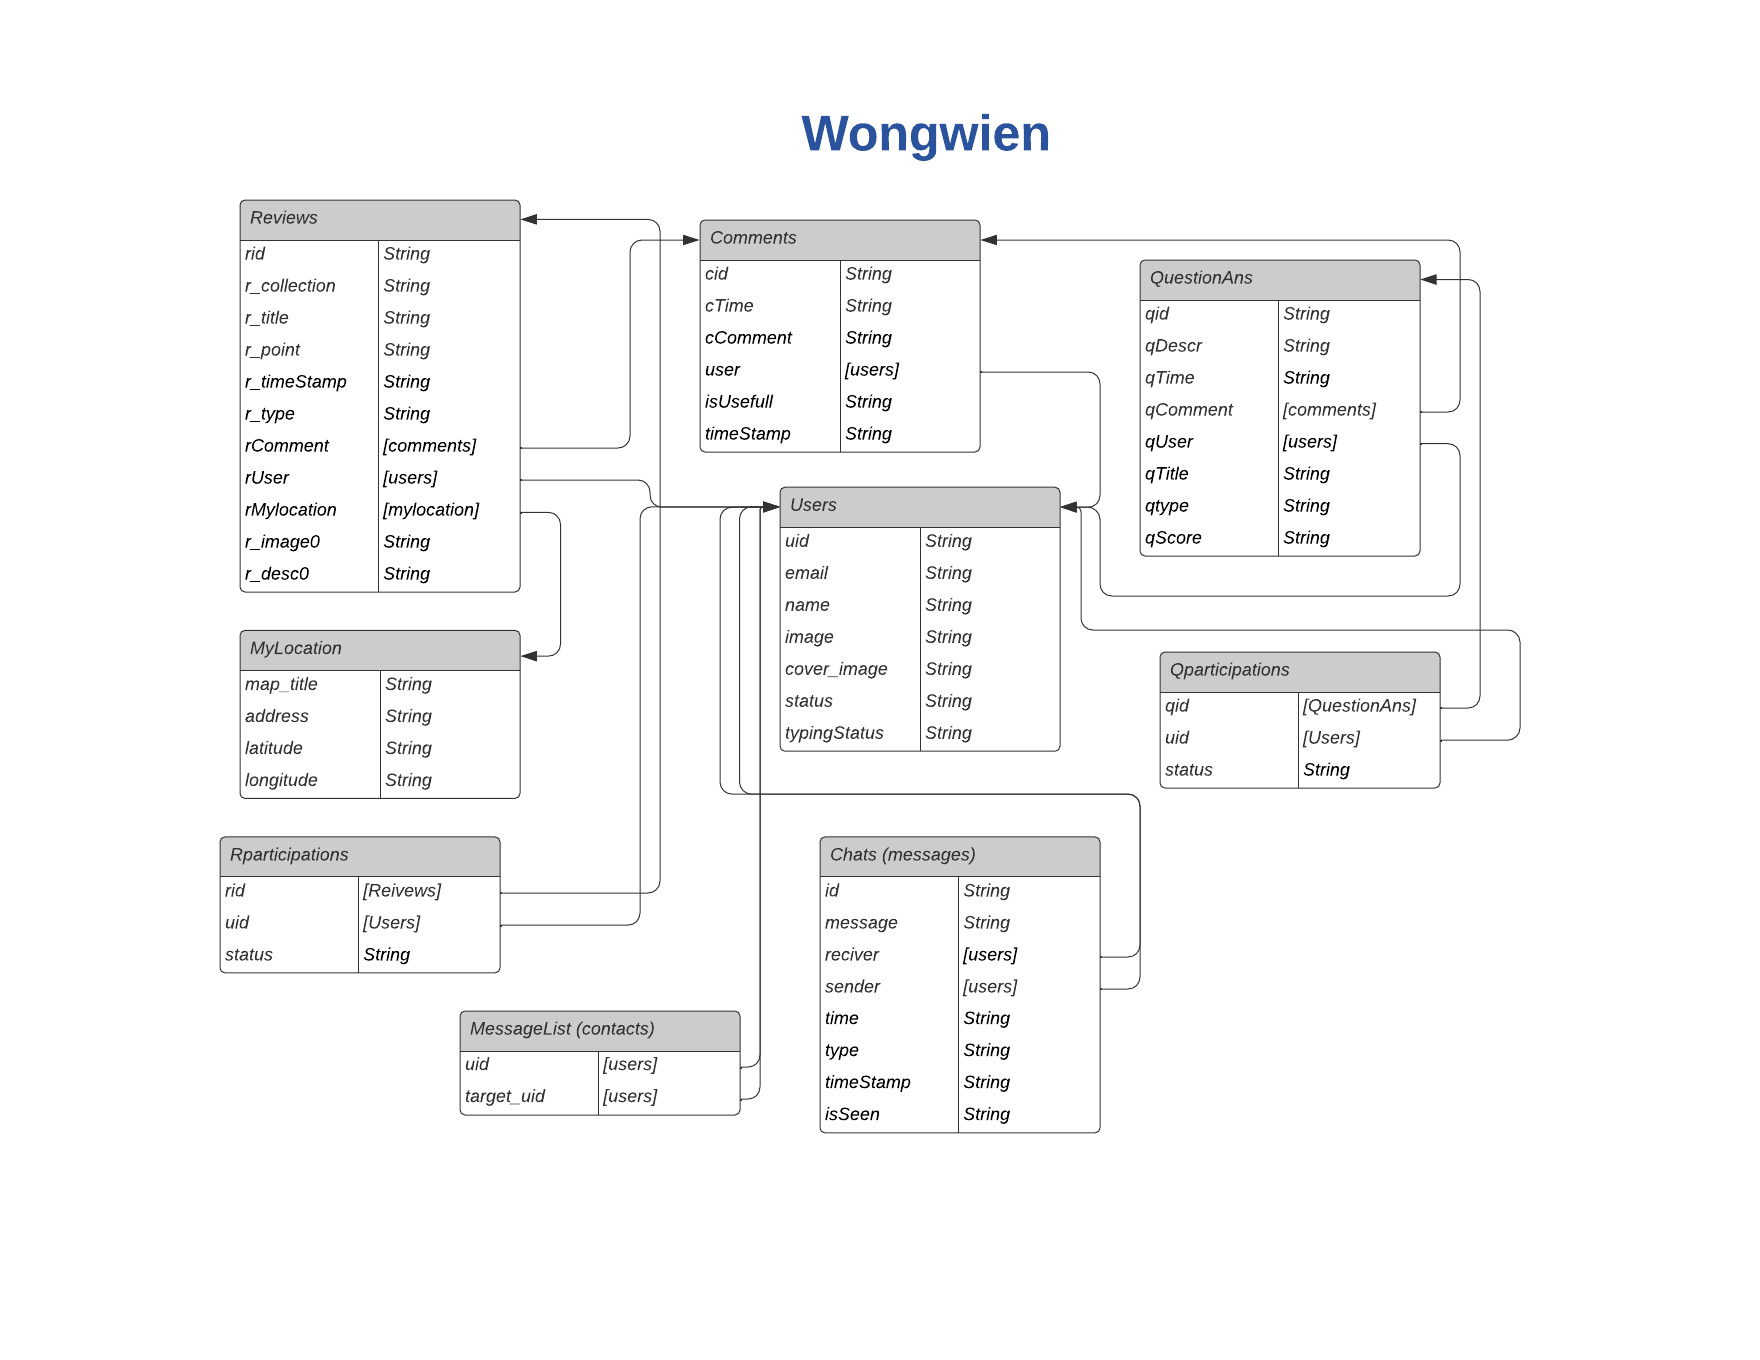
\includegraphics[width=1\textwidth]{./image/database.jpeg}
  \end{center}
  \caption[Poem]{System architecture}
  \end{figure}


\section{โครงสร้างของแอปพลิเคชัน}
\subsection{Use case diagram}

